% Copyright 2026 Sreeram Anil
% SPDX-License-Identifier: CC-BY-4.0
% =============================================================================
%  Plain (linearised-once) Kalman filter — classical Kalman family
% =============================================================================
\chapter{Linear Kalman Filter on a Frozen Linearisation (LKF)}
\label{ch:lkf}

\section*{At a glance}
\begin{tabular}{@{}l>{\raggedright\arraybackslash}p{0.76\textwidth}@{}}
Family & classical Kalman \\
Header & \texttt{include/estkit/filters/kf\_linear.hpp} \\
Registered name & \texttt{LKF} \\
State dimension & $n_x = 4$ (cell model) --- generic in $n_x, n_u, n_y$ \\
Cost per step & $\mathcal{O}(n_x^3)$, $320$--$336$\,ns/step; gain schedule computable offline \\
Primary references & \cite{kalman1960,kalmanbucy1961,andersonmoore1979,sorenson1970gauss} \\
\end{tabular}

\section{Motivation and aerospace/BMS relevance}
Kalman's 1960 filter is optimal for a \emph{linear} system. Everything else in this report is
an attempt to keep that optimality in the presence of nonlinearity. It is therefore worth
establishing, quantitatively, what happens if one simply ignores the problem: linearise the
cell model once, at power-up, and run the textbook linear filter for the rest of the flight.

This is not a straw man. A time-invariant Kalman filter has properties no nonlinear filter
can offer. Its Riccati recursion does not depend on the data, so $\mP_k$ and $\mK_k$ can be
computed on the ground and stored as a table --- or replaced by their steady-state values
$\mP_\infty, \mK_\infty$, the solution of a discrete algebraic Riccati equation
\cite[\S4.4]{andersonmoore1979}. The flight code is then a fixed-gain observer costing
$n_x n_y$ multiplies per step, with no matrix inversion, no Cholesky, no Jacobian evaluation
and a completely deterministic execution time --- the kind of code that gets certified
quickly. Several production BMS use exactly this structure with a gain scheduled on
temperature. The question this chapter answers is what it costs in accuracy.

\section{Problem statement and assumptions}
The plant is \eqref{eq:ekf-proc}--\eqref{eq:ekf-meas}. The filter is given, once, a
linearisation point $(\vx_0,\vu_{\text{lin}})$ --- in the benchmark the initial estimate and
the cell at rest, $\vu_{\text{lin}} = [0, T_0]^\T$ with $T_0$ the temperature reported at
reset --- and forms the constant matrices
\begin{equation}
\mF = \left.\frac{\partial f}{\partial\vx}\right|_{\vx_0,\vu_{\text{lin}}}, \qquad
\mH = \left.\frac{\partial h}{\partial\vx}\right|_{\vx_0,\vu_{\text{lin}}}, \qquad
\mQ = \mQ(\vx_0,\vu_{\text{lin}}), \qquad
\mR = \mR(\vx_0,\vu_{\text{lin}}).
\label{eq:lkf-frozen}
\end{equation}
\begin{assumption}[Global linearity about one point]\label{as:lkf}
The first-order Taylor expansions of $f$ and $h$ about $\vx_0$ are accurate over the whole
trajectory the state will visit, and the noise statistics do not depend on the operating
point.
\end{assumption}
Assumption~\ref{as:lkf} is much stronger than the EKF's Assumption~\ref{as:ekf-lin} and is,
for a battery discharging from $95\,\%$ to $20\,\%$ SOC, plainly false. Quantifying ``how
false'' is the purpose of the experiment.

\section{Derivation}
Write the affine surrogate model obtained by freezing the Jacobians but keeping the exact
dependence on the (measured) input:
\begin{align}
f(\vx,\vu) &\approx \tilde f(\vx,\vu) := f(\vx_0,\vu) + \mF(\vx - \vx_0), \label{eq:lkf-f}\\
h(\vx,\vu) &\approx \tilde h(\vx,\vu) := h(\vx_0,\vu) + \mH(\vx - \vx_0). \label{eq:lkf-h}
\end{align}
Both are exact in $\vu$ and first order in $\vx$ about $\vx_0$; in particular the
ampere-hour integration and the ohmic term $-R_0(T)i$ are reproduced exactly, so the
surrogate is not a caricature but a genuine linear time-varying-input model. The Kalman
recursion for \eqref{eq:lkf-f}--\eqref{eq:lkf-h} is
\begin{align}
\xminus_k &= \mF\left(\xplus_{k-1} - \vx_0\right) + f(\vx_0, \vu_{k-1}), &
\Pminus_k &= \mF\Pplus_{k-1}\mF^\T + \mQ, \label{eq:lkf-tu}\\
\yhat_k &= h(\vx_0,\vu_k) + \mH(\xminus_k - \vx_0), &
\mS_k &= \mH\Pminus_k\mH^\T + \mR, \label{eq:lkf-ypred}\\
\mK_k &= \Pminus_k\mH^\T\mS_k\inv, &
\xplus_k &= \xminus_k + \mK_k(\vy_k - \yhat_k), \label{eq:lkf-gain}
\end{align}
with the Joseph covariance update \eqref{eq:ekf-joseph}. Because $\mF,\mH,\mQ,\mR$ are
constant, the pair $(\Pminus_k,\mK_k)$ obeys the deterministic Riccati recursion
\begin{equation}
\Pminus_{k+1} = \mF\left[\Pminus_k - \Pminus_k\mH^\T(\mH\Pminus_k\mH^\T+\mR)\inv \mH\Pminus_k\right]\mF^\T + \mQ,
\label{eq:lkf-riccati}
\end{equation}
which, if $(\mF,\mH)$ is detectable and $(\mF,\mQ^{1/2})$ stabilisable, converges to the
unique stabilising solution $\mP_\infty$ of the DARE and the gain to
$\mK_\infty = \mP_\infty\mH^\T(\mH\mP_\infty\mH^\T+\mR)\inv$
\cite[Ch.~4]{andersonmoore1979}. For the cell model $\mF=\diag(1,a_1,a_2,a_h)$ and
$\mH=[\partial\ocv/\partial\soc,\,-1,\,-1,\,M]$; the pair is observable because the first
entry of $\mH$ is non-zero, so the SOC integrator is stabilised through the OCV channel.
\code{estkit} provides \code{dare\_iterate} for the offline computation of
$(\mP_\infty,\mK_\infty)$.

\paragraph{The error this introduces.} The measurement bias committed at state $\vx$ is
\begin{equation}
b(\vx) = h(\vx,\vu) - \tilde h(\vx,\vu) = \ocv(\soc) - \left[\ocv(\soc_0) + \ocv'(\soc_0)(\soc-\soc_0)\right]
 = \tfrac12 \ocv''(\xi)(\soc-\soc_0)^2
\label{eq:lkf-bias}
\end{equation}
for some $\xi$ between $\soc_0$ and $\soc$ --- the deviation of the OCV curve from its
tangent at the linearisation point, not merely the slope error. A persistent measurement
bias $b$ is absorbed by a steady-state SOC error of approximately
$\Delta\soc \approx -b/\ocv'$, since in steady state the filter drives the innovation to
zero. This is the dominant error mechanism of the LKF and it grows quadratically as the cell
discharges away from $\soc_0$.

\section{Algorithm}
\begin{algorithm}[H]
\caption{LKF --- initialisation and one sampling period}
\begin{algorithmic}[1]
\Require at reset: $\vx_0, \mP_0, \vu_{\text{lin}}$
\State \textbf{Once:} $\mF\gets \partial f/\partial\vx|_{\vx_0,\vu_{\text{lin}}}$,\;
       $\mH\gets \partial h/\partial\vx|_{\vx_0,\vu_{\text{lin}}}$,\;
       $\mQ\gets\mQ(\vx_0,\vu_{\text{lin}})$,\; $\mR\gets\mR(\vx_0,\vu_{\text{lin}})$
\State \textbf{Time update:} $\xminus_k\gets f(\vx_0,\vu_{k-1}) + \mF(\xplus_{k-1}-\vx_0)$
\State $\Pminus_k \gets \mF\Pplus_{k-1}\mF^\T+\mQ$; symmetrise
\State \textbf{Predicted measurement:} $\yhat_k \gets h(\vx_0,\vu_k) + \mH(\xminus_k-\vx_0)$
\State \textbf{Measurement update:} $\mS\gets\mH\Pminus_k\mH^\T+\mR$,\;
       $\mK\gets\Pminus_k\mH^\T\mS\inv$
\State $\xplus_k\gets\xminus_k+\mK(\vy_k-\yhat_k)$,\;
       $\Pplus_k\gets(\mI-\mK\mH)\Pminus_k(\mI-\mK\mH)^\T+\mK\mR\mK^\T$
\State \textbf{if} constraints enabled \textbf{then} $\xplus_k\gets\Pi(\xplus_k)$
\Ensure $\xplus_k,\Pplus_k$; \quad (steps 3, 5 may be replaced by the stored $\mK_\infty$)
\end{algorithmic}
\end{algorithm}

\section{Application to the battery model}
The frozen quantities for the nominal benchmark are, at $\soc_0=0.95$, $T_0=298.15$\,K and
$i=0$:
\begin{equation}
\mF = \diag(1,\;0.9802,\;0.99917,\;1), \qquad
\mH = [\,0.7485,\;-1,\;-1,\;0.005\,].
\label{eq:lkf-battery}
\end{equation}
Two entries deserve comment. $\mH_{1}=\partial\ocv/\partial\soc$ at $\soc=0.95$ is
$0.7485$\,V, while over the mission the true slope ranges from $0.71$\,V at $\soc=0.4$ to
$0.93$\,V at $\soc=0.8$ --- a modest $\pm 20\,\%$, so the \emph{slope} alone is not the
problem. The tangent-line \emph{offset} \eqref{eq:lkf-bias} is: integrating the curvature
from $\soc_0 = 0.95$ down to $\soc = 0.20$ accumulates a model voltage error of order
$40$\,mV, i.e. $\Delta\soc \approx 0.05$. Second, $a_h(i{=}0) = 1$: linearising at rest
freezes the hysteresis state as a pure random walk, so its decay is lost.

The \code{u\_lin} option is set by the registry to $[0, T_0]^\T$, i.e. the cell at rest at
the temperature reported at reset; \code{freeze\_noise = true} gives the strictly
time-invariant filter described above (setting it to \code{false} re-evaluates $\mQ,\mR$ at
the current input and was measured to change nothing at all on this benchmark, to four
decimal places, in all scenarios).

\section{Implementation notes}
The implementation keeps $\vx_0$, $\mF$, $\mH$, $\mQ$, $\mR$ as members, so the per-step work
is two $4\times4$ products and one $1\times1$ inverse: $320$--$336$\,ns, the cheapest filter of the
fifteen and $\approx 30\,\%$ faster than the EKF ($443$--$482$\,ns), which must rebuild $\mF$
and $\mH$ every step. \code{sizeof(LinearKf<EcmModel>)} is 4680\,bytes, again dominated by the model copy.
Because $\mP_k$ follows \eqref{eq:lkf-riccati} independently of the data, a flight
implementation would drop $\mP$ entirely and store $\mK_\infty$ (four reals), reducing the
filter to $\xplus = \xminus + \mK_\infty \veps$ --- 4 multiply-accumulates per step. The
float build reproduces the double results exactly to four decimals in every scenario, as
expected for a filter whose covariance never becomes ill-conditioned.

\section{Benchmark results}
% Copyright 2026 Sreeram Anil
% SPDX-License-Identifier: CC-BY-4.0
\begin{table}[H]\centering\footnotesize\setlength{\tabcolsep}{4pt}
\caption{LKF: cell-level benchmark on the eVTOL mission (mean over seeds; RMSE and max error in \% SOC; $t_\mathrm{conv}$: first time the error stays below 2\,\% for 60\,s, -- = never; EKF reference: steady-state RMSE of the plain EKF on the same data).}\label{tab:cell_LKF}
\begin{tabular}{llrrrrrcrr}\toprule
plant & scenario & RMSE & RMSE$_\mathrm{ss}$ & max & $t_\mathrm{conv}$ [s] & RMSE$_v$ [mV] & div. & EKF ref. & ns/step \\ \midrule
ECM & nominal & 3.23 & 1.19 & 6.29 & 0 & 1.13 & no & 0.05 & 334 \\
ECM & init\_error & 3.44 & 2.19 & 6.01 & 0 & 2.24 & no & 0.05 & 332 \\
ECM & current\_bias & 3.74 & 1.36 & 7.15 & 0 & 1.13 & no & 0.61 & 335 \\
ECM & noise\_step & 3.23 & 1.19 & 6.29 & 0 & 2.98 & no & 0.12 & 332 \\
ECM & outliers & 3.24 & 1.19 & 6.41 & 0 & 2.20 & no & 0.21 & 331 \\
ECM & cold & 13.12 & 12.49 & 18.93 & 0 & 3.86 & no & 0.16 & 330 \\
ECM & hot & 2.14 & 1.62 & 3.91 & 0 & 1.02 & no & 0.03 & 329 \\
ECM & aged\_cell & 1.67 & 1.14 & 5.64 & 0 & 4.05 & no & 1.52 & 330 \\
ECM & param\_mismatch & 1.81 & 1.19 & 3.63 & 0 & 2.90 & no & 1.36 & 332 \\
ECM & sensor\_dropout & 3.27 & 1.20 & 6.34 & 0 & 1.75 & no & 0.46 & 330 \\
ECM & preisach & 2.76 & 1.06 & 5.40 & 0 & 1.11 & no & 0.20 & 336 \\
ECM & combined & 6.38 & 7.00 & 11.89 & -- & 5.16 & no & 12.44 & 331 \\
\midrule
SPM & nominal & 1.30 & 1.72 & 2.71 & 0 & 1.05 & no & 3.73 & 330 \\
SPM & init\_error & 0.56 & 0.55 & 1.27 & 0 & 2.18 & no & 3.81 & 321 \\
SPM & current\_bias & 1.96 & 2.65 & 4.06 & 0 & 1.12 & no & 5.69 & 324 \\
SPM & noise\_step & 1.30 & 1.72 & 2.84 & 0 & 3.15 & no & 3.30 & 327 \\
SPM & outliers & 1.30 & 1.71 & 2.81 & 0 & 2.27 & no & 1.99 & 322 \\
SPM & cold & 1.70 & 1.47 & 4.19 & 256 & 4.60 & no & 7.35 & 320 \\
SPM & hot & 1.27 & 1.44 & 2.61 & 0 & 0.74 & no & 2.16 & 326 \\
SPM & param\_mismatch & 2.23 & 2.86 & 4.20 & 0 & 1.95 & no & 3.13 & 325 \\
SPM & sensor\_dropout & 1.30 & 1.70 & 2.99 & 0 & 1.92 & no & 5.31 & 324 \\
\bottomrule\end{tabular}\end{table}

\begin{figure}[H]\centering
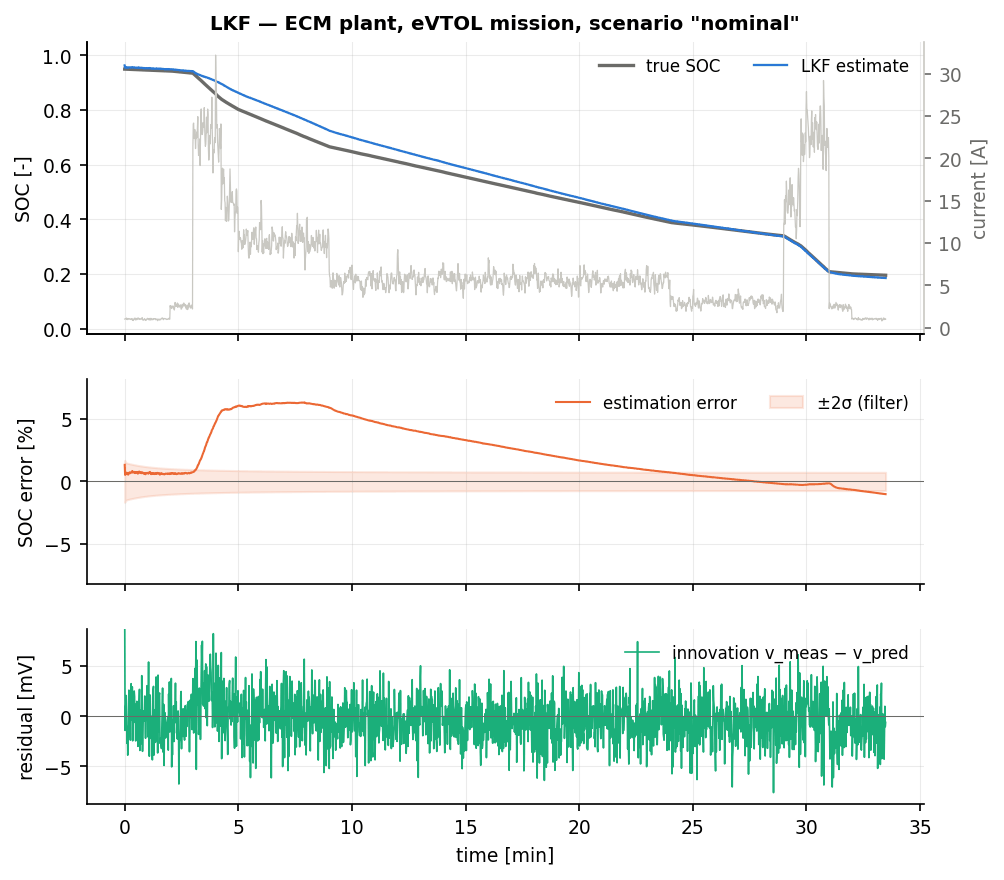
\includegraphics[width=\textwidth]{figures/cell_LKF_nominal.png}
\caption{LKF on the nominal eVTOL mission: true and estimated SOC (top), estimation error with the $\pm 2\sigma$ band when available (middle), voltage residual (bottom).}
\end{figure}
\begin{figure}[H]\centering
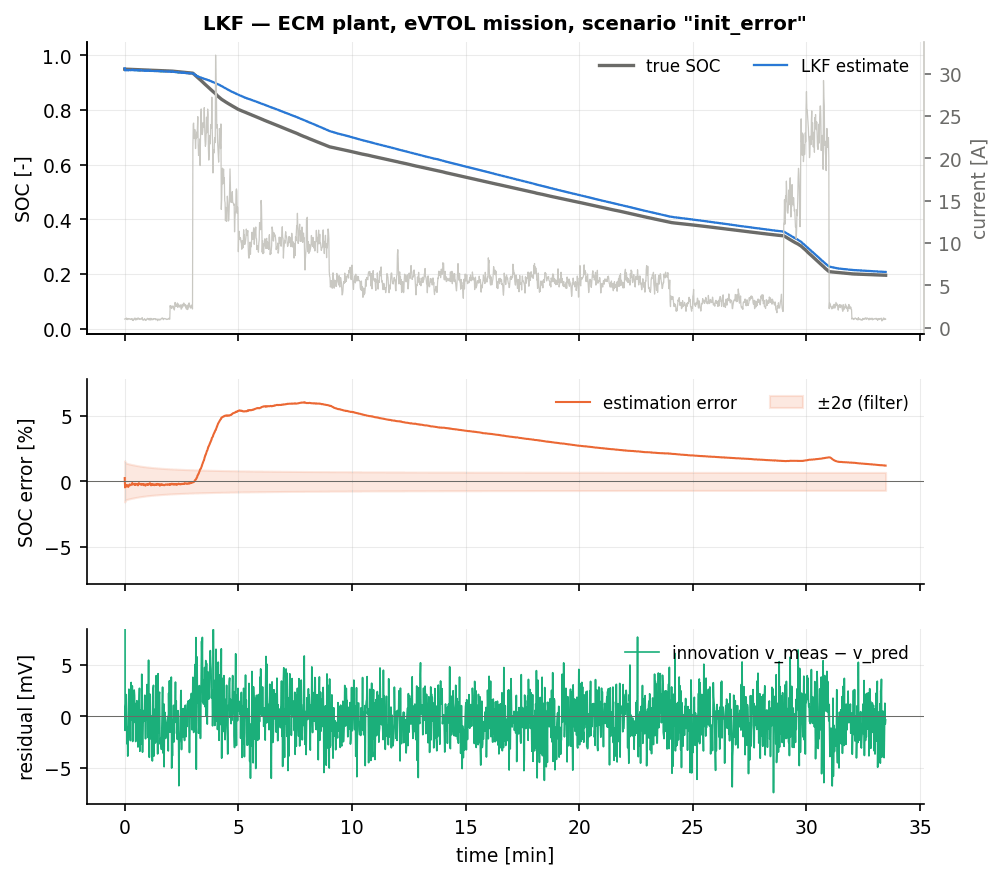
\includegraphics[width=\textwidth]{figures/cell_LKF_init_error.png}
\caption{LKF with a 35\,\% initial SOC error.}
\end{figure}

All numbers are three-seed means in per cent SOC.

The headline number is $\text{RMSE}_{\text{ss}} = 1.19\,\%$ on \texttt{nominal} against the
EKF's $0.05\,\%$: freezing the linearisation costs a factor of twenty-four in steady-state
accuracy, and the whole-run RMSE ($3.23\,\%$ against $0.15\,\%$) a factor of twenty-one. The
filter still converges from the $-35\,\%$ initial error in a single sample, because the gain
computed from $\mP_0$ is large and the frozen $\mH$ has the right sign and roughly the right
magnitude. What it cannot do is track: the error signature in the nominal figure is a slow
drift that follows the deviation of the OCV curve from its tangent, exactly as predicted by
\eqref{eq:lkf-bias}, with a maximum error of $6.29\,\%$. The voltage residual RMSE,
$1.13$\,mV against the EKF's $0.79$\,mV, shows the same bias in the measurement channel. Note
that the whole-run RMSE exceeds the acceptance threshold on several scenarios even though the
steady-state figure does not; the LKF is a filter whose transient is its best part.

\texttt{cold} is the clearest failure: $\text{RMSE}_{\text{ss}} = 12.49\,\%$, ten times worse
than nominal and eighty times worse than the EKF's $0.16\,\%$. The cause is not the OCV but the
frozen RC pole. At $T_0 = 263$\,K the model gives $\tau_1 = 19.1$\,s, hence $a_1 = 0.99477$;
the cell self-heats to $\approx 275$\,K during the mission, where the true $a_1 = 0.99147$.
Since the steady-state RC voltage of the frozen model is
$R_1(T)(1-a_1(T))\,i/(1-a_1^{\text{frozen}})$, the ratio
$(1-a_1^{\text{true}})/(1-a_1^{\text{frozen}}) = 1.63$ means $v_1$ is overestimated by
$63\,\%$ --- and at $22$\,A with a cold $R_1 = 23$\,m$\Omega$ that is a $0.3$\,V error in the
predicted terminal voltage, which the filter can only remove by biasing SOC by
$0.3/0.8\approx 0.19$. An EKF evaluates $a_1(T_k)$ every step and does not have this problem
at all.

\texttt{combined} gives $7.00\,\%$ and never converges; \texttt{init\_error} settles at
$2.19\,\%$ (the frozen tangent is taken at $\soc_0 = 0.60$ there, which fits the lower half of
the OCV curve worse than the tangent at $0.95$ fits the upper half); \texttt{hot} $1.62\,\%$.
Everything else sits at the $1.1$--$1.4\,\%$ tangent-line floor, essentially independent of the
scenario --- \texttt{noise\_step}, \texttt{outliers} and \texttt{sensor\_dropout} are all
$1.19$--$1.20\,\%$, i.e. the LKF does not notice them. \texttt{preisach} is $1.06\,\%$ and
now converges in the first sample, where before the plant's hysteresis sign was corrected it
took over $1300$\,s. As on the ECM plant generally, the LKF is \emph{better} than the EKF on
\texttt{aged\_cell} ($1.14\,\%$ against $1.52\,\%$) and \texttt{param\_mismatch} ($1.19\,\%$
against $1.36\,\%$); that is not a property of the method but a consequence of its low fixed
gain, which is also what makes the SPM result below so striking.

\paragraph{SPM plant: structured model error, and why the LKF wins it.}
\begin{figure}[H]\centering
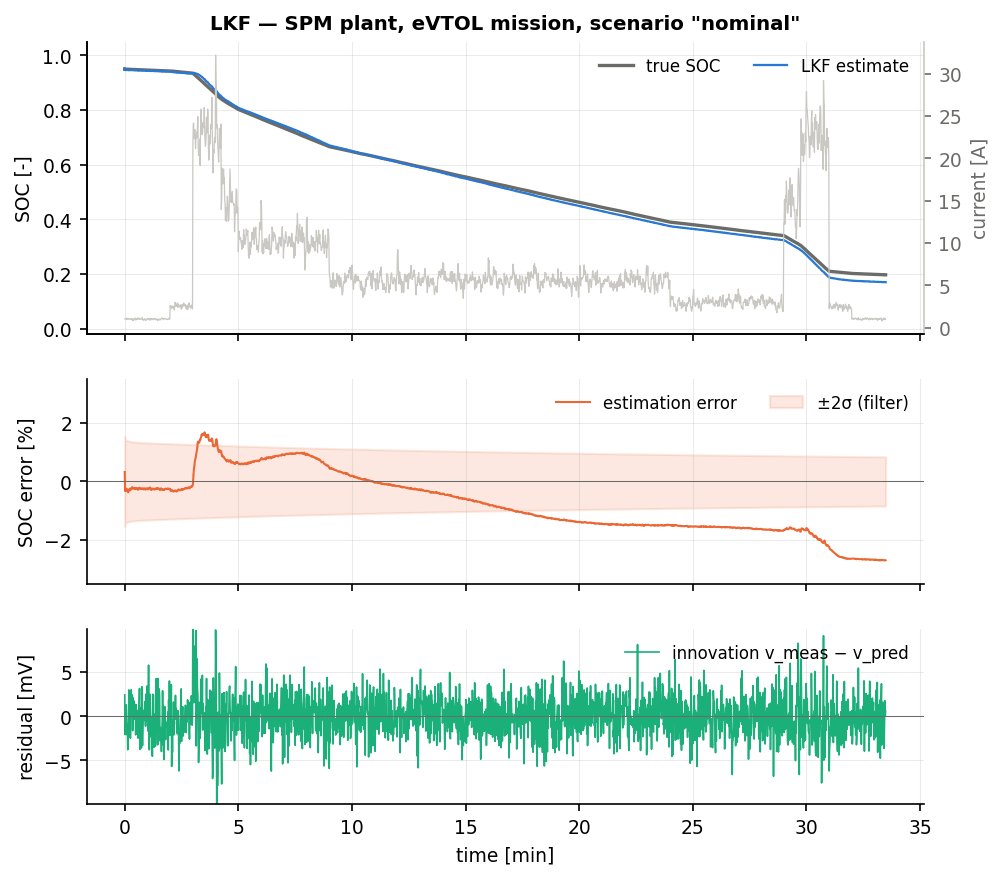
\includegraphics[width=\textwidth]{figures/cellspm_LKF_nominal.png}
\caption{LKF on the nominal mission with the electrochemical (SPM) plant: the frozen gain keeps the estimate close to ampere-hour integration and away from the badly conditioned OCV channel.}
\end{figure}
The SPM block of the table is a different kind of test. The plant is the electrochemical
single-particle model; the estimator still runs a 2-RC equivalent circuit, fitted to that plant,
which leaves a \emph{structured} residual of about $4$\,mV (Butler--Volmer kinetics and
solid-phase diffusion that no 2-RC circuit can reproduce) and a slow second branch,
$\tau_2 = 556$\,s. Over a $33$-minute mission a $556$\,s pole barely relaxes, so $v_2(t)$ is
close to an affine ramp --- and so is $\ocv(\soc(t))$ while the cell discharges at a roughly
constant rate. The two channels through which the measurement sees the state,
$(\partial\ocv/\partial\soc)\,\delta\soc$ and $-\delta v_2$, are therefore nearly collinear in
the information accumulated over the flight: the pair $(\soc, v_2)$ is close to unobservable,
and no filter can decide whether a persistent few-millivolt residual belongs to the slow RC
branch or to the state of charge. Because that direction is weakly observable, a $4$\,mV
structured error maps onto \emph{several per cent} of SOC instead of the
$4\,\text{mV}/0.8\,\text{V}\approx0.5\,\%$ a well-conditioned channel would give. This
$(\soc,v_2)$ ambiguity, not the size of the residual, is the mechanism behind the
$3.7$--$4.6\,\%$ band in which the whole classical family sits.

The LKF is the exception, and by a wide margin: $1.72\,\%$ on SPM \texttt{nominal} against
$3.73\,\%$ for the EKF, $3.96\,\%$ for the UKF and $4.62\,\%$ for the cubature filters, and
$1.47\,\%$ on SPM \texttt{cold} where every other filter in the family is between $7.4$ and
$8.7\,\%$. It is the only member of the family whose SPM performance is no worse than its ECM
performance ($1.72\,\%$ against $1.19\,\%$), and on SPM \texttt{init\_error} it reaches
$0.55\,\%$ --- its best result anywhere in this report.

The explanation is the same rigidity that costs it a factor of twenty on the ECM plant. Its
measurement model is the tangent frozen at $\soc_0$, so it never tracks the OCV slope as the
cell discharges, and the gain along the ill-conditioned $(\soc, v_2)$ direction is fixed once
by the Riccati recursion \eqref{eq:lkf-riccati} rather than re-derived at every step from a
Jacobian that the SPM residual has corrupted. Where an EKF confidently re-linearises and
re-apportions the $4$\,mV residual between $\soc$ and $v_2$ --- committing, step after step, to
a split that the data cannot support --- the LKF simply has no mechanism for doing so. It
therefore stays much closer to open-loop ampere-hour integration, which on the SPM plant is
nearly exact because the current record is clean, and declines to pump the structured residual
into SOC. The $0.55\,\%$ on SPM \texttt{init\_error} is the same effect seen from the other
side: linearising at $\soc_0 = 0.60$ happens to place the frozen tangent where the SPM's true
OCV mapping is best matched.

This is a cautionary result, not a recommendation. The LKF is not modelling the SPM plant
better than the EKF --- it is modelling it worse, and being saved by a low, fixed gain that
keeps it from acting on a corrupted correction. The principled versions of the same idea are a
deliberately de-weighted OCV channel (a larger $\mR$), an $H_\infty$ gain, or an augmented
state that gives the structured residual somewhere to go.

\section{Summary}
The frozen-linearisation Kalman filter is the cheapest member of the family
($320$--$336$\,ns/step, a precomputable gain, no run-time Jacobians) and it converges and
remains stable on every scenario of both plants. It costs a factor of twenty-four in
steady-state SOC accuracy on the nominal ECM mission and fails outright when the operating
point moves far from the linearisation point in \emph{temperature}, because the frozen RC poles
then describe the wrong cell. Its one genuine success is the SPM plant, where its low fixed
gain makes it the most accurate filter of the family under structured model error --- for the
wrong reason. Use it only where the SOC window and the temperature are both narrow and a
$1$--$2\,\%$ SOC error is acceptable; for anything resembling a full discharge, re-linearising
every step costs $140$\,ns more and is twenty times more accurate.
